\chapter[Survey]{Survey of Existing Work}

This chapter aims to give an overview of the existing work that tackles the problem of querying structured knowledge bases. As we discussed in Chapter 1, the use of structured query languages (e.g. SPARQL) is limited by requirement that the user must be aware of schema of the queried data. We will see in this chapter multiple approaches that seek to remedy that. A full coverage and critique of all approaches is beyond the scope of this report, so we shall select a few interesting ones for the purpose of this chapter. The approaches will be organized by their central ideas.

\section[Keyword Queries]{Free-Keyword Querying}
 
 In \cite{elbassuoni2011keyword}, the authors develop a retrieval model that enables users to search RDF graphs using keywords. In contrast to approaches that retrieve entity tuples, the model here returns a ranked list of RDF \emph{subgraphs}. Retrieving subgraphs allows the treatment of triples in a holistic manner by explicitly taking into account the relationships between entities.
 
 To process keyword queries over RDF graphs, the system associates each triple $t_i$ with a set of keywords derived from the subject and object of the triple, as well as representative keywords for the predicate and constructs a document $D_i$. The terms in the document $D_i$ are stemmed using any standard stemmer and then stored in an inverted index. In addition, the term frequency of term $w$ in $D_i$, referred to as $c(w, D_i)$, is also stored.
 
 The first step towards query processing is to retrieve a set of subgraphs that match the user keyword query. To avoid retrieving large and noisy subgraphs, the following constraints are imposed: 1) the subgraphs should be unique and maximal (no subgraph should be a subset of any other subgraph retrieved), and 2) the subgraphs should contain triples matching different sets of keywords (no triples in the same subgraph should match the exact same set of keywords). The rationale behind the latter constraint is that if two triples match the same set of keywords, they are parts of two different possible results to the user query, and should be considered as parts of two separate subgraphs.
 
 Let the keyword query be $q = \{q_1, q_2, ..., q_m\}$, the subgraph-retrieval algorithm utilizes the inverted index to retrieve lists $\{L_1, L_2, ..., L_m\}$. The set $E$ of all unique triples in all lists can be viewed as a disconnected graph\footnote{each triple can be viewed as an edge where its subject  and object are nodes} and is referred to as the query graph. An adaptation of the network-motif detection algorithm \cite{wernicke2005faster} is used on $E$ to retrieve the desired subgraphs. We omit the discussion here.
 
 On retrieving a set of subgraphs matching a given keyword query, the next step is to rank these subgraphs. The ranking model is based on statistical language model techniques \cite{ponte1998language}. Given a subgraph $G = \{t_1, t_2, ..., t_n\}$, where $t_i$ is a triple, and the query $q = \{q_1, q_2, ..., q_m\}$ where $q_i$ is a single term, the subgraph G  is ranked based on the probability of generating the query Q given the subgraph $G$'s language model. Independence is assumed between the query terms, and likelihood $\text{Pr}(q|G)$ is computed as:
 $$ \text{Pr}(q|G) = \prod_{i=1}^{m} \text{Pr}(q_i|G)$$
 where $\text{Pr}(q_i|G)$ denotes the probability of term $q_i$ in the language model of $G$. The language model of subgraph $G$ is computed as a mixture model of the language models of its constituent triples, 
 
 $$ \text{Pr}(q_i|G) = \frac{1}{n} \sum_{j=1}^{n} \text{Pr}(q_i|t_j)$$

 where $\text{Pr}(q_i | t_j)$ is computed from the document $D_j$ constructed earlier.
 
 The performance of the above model is compared with well-known techniques for keyword search over structured data \cite{bhalotia2002keyword, nie2007web} and we refer the interested reader to the original paper \cite{elbassuoni2011keyword} for that.
 
 
\section{Converting queries to SPARQL}

DEANNA \cite{yahya2012deep} is a framework for natural language question answering over structured knowledge bases. The approach followed by DEANNA is to convert the natural language question to an appropriate SPARQL query that can be then processed over the knowledge base. By far, the main challenge addressed is that of disambiguating user intent expressed in the verbal phrases and noun phrases in the question, and doing this in a globally coherent manner.

As a first step, phrases are detected in the natural language question that potentially correspond to semantic items. This phrase detector unit uses multiple detectors, each of which can detect a certain class of phrases, corresponding to semantic classes, entities, relations and interrogative pronouns. The detectors utilize different named entity recognition and relation detection techniques.

Next, the system attempts to detect \emph{triploids} in the natural language question. A triploid are 3-tuple of tokens which corresponds to a relation and its two arguments. These triploids and the candidate phrases from the previous step are are consolidated into \emph{q-units}, which are phrase-level triples (can possibly have multiple candidates for a relation and arguments).

\begin{figure}
  \center
  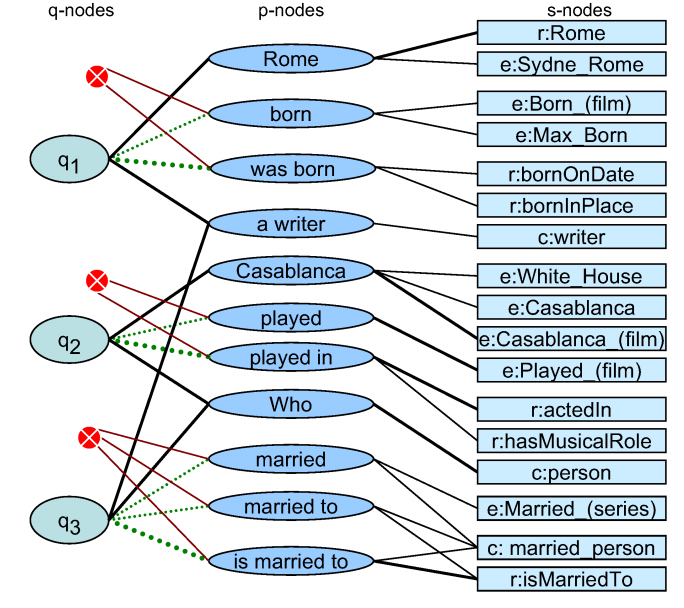
\includegraphics[scale=0.5]{./deanna1.png}
  \label{fig:disgraph}
  \caption{Disambiguation graph. Attribution: \cite{yahya2012deep}}
\end{figure}

The next (and probably the most interesting) step is to perform disambiguation to resolve the mappings of phrases to semantic items. This is done in a joint manner---a weighted disambiguation graph is constructed and a dense subgraph is sought. A disambiguation graph (Figure \ref{fig:disgraph}) is a 3-partite graph with weighted edges. The edge weights are given as a combination of semantic coherence and syntactic similarity. Q-nodes collect triples of phrases together and this can been seen as dotted edges in Figure \ref{fig:disgraph}. 

The problem of disambiguation now translates to finding a dense subgraph in the disambiguation graph. The density measure is a function of edge weights (which measure syntactic similarity and semantic coherence). Further constraints are put on the subgraph such that it represents a valid triple. The objective and the constraints are encoded as an integer linear program and fed into an ILP solver---which then returns the required subgraph.

Once the disambiguation is completed, semantic grouping is performed which forms semantic triples. For example, if it is determined that the relation \texttt{marriedTo} connects the person referred to by `Who' and the \texttt{writer} to form the semantic triple \texttt{person marriedTo writer}. These semantic triples are transformed into SPARQL queries using a rule based method. For example, \texttt{person marriedTo writer} is transformed to \texttt{?x type person}, \texttt{?x marriedTo ?w}, \texttt{?w type writer}.

%---------------GQBE Start----------------------------

\section{Querying by example entity tuples}


 GQBE \cite{jayaram2013querying} proposes to query knowledge graphs by example entity tuples. The user input and output of GQBE are both entity tuples,
called query tuples and answer tuples, respectively. Plainly stated, given a data graph $G$ and a query tuple $t$, GQBE tries to find the top-$k$ answer tuples $t'$ with the highest similarity scores $\text{score}_t(t')$.
 
 
 $\text{score}_t(t')$ is computed by matching the inter-entity relationships of $t$ and that of $t'$. Matching is not done on an entity-level in $t$, rather, a neighborhood graph is constructed (captures `features' that might be of interest to users) from $t$ and $\text{score}_t(t')$ entails matching two
 graphs constructed from $t$ and $t'$ respectively.
 
 The neighborhood graph $H_t$ of an example tuple $t$ is a weakly connected undirected subgraph of $G$ (the data graph) consisting of all nodes reachable from nodes of $t$ by an undirected path of length less than a user defined threshold $d$.
 
 It is observed that $H_t$ can be enormously large even for small values of $d$ (800K nodes for $d = 2$ in case of Freebase). Therefore, GQBE constructs a Maximum Query Graph (MQG) from $H_t$ which is expected to be drastically smaller than $H_t$ and yet capturing important features of the query tuple. $MQG_t$, given
 a parameter $m$, is a weakly connected subgraph of the  neighborhood graph $H_t$ that maximizes total edge weight
 $\sum_e w(e)$ while satisfying the constraints that it contains all the nodes in $t$, and contains at most $m$ edges.
 
 The decision version of finding $MQG_t$ for a given $m$ is shown to be NP-hard, and therefore GQBE employs a greedy algorithm to get an approximate $MQG_t$.
 
 Given a $MQG_t$, the goal is to find answer graphs $A$ which have high similarity to $MQG_t$. An answer graph $A$ to a query graph $Q$ is a
 weakly connected subgraph of $G$ that is edge-isomorphic to $Q$. Similarity is defined as a composite of a content-score and a structure-score. Structure-score captures measures the important structure in $MQG_t$ that is captured by $Q$. Content-score is defined by giving extra credit for identical nodes among the matching nodes in answer graph $A$ and query graph $Q$.
 
 Finally, GQBE searches $G$ for the top-$k$ answer subgraphs (according to the similarity score) in a best-first manner. We omit the algorithm in this discussion. 
 
 \section{Interactive Queries}
 
 Next, we cover FreeQ \cite{demidova2012freeq} - an interactive interface for incremental query construction. It enables a user to start with simple keywords and incrementally refine them into a structured query that captures the user's information need. Figure \ref{fig:freeq} illustrates the FreeQ user interface.

 \begin{figure}[h!]
 %\centering
 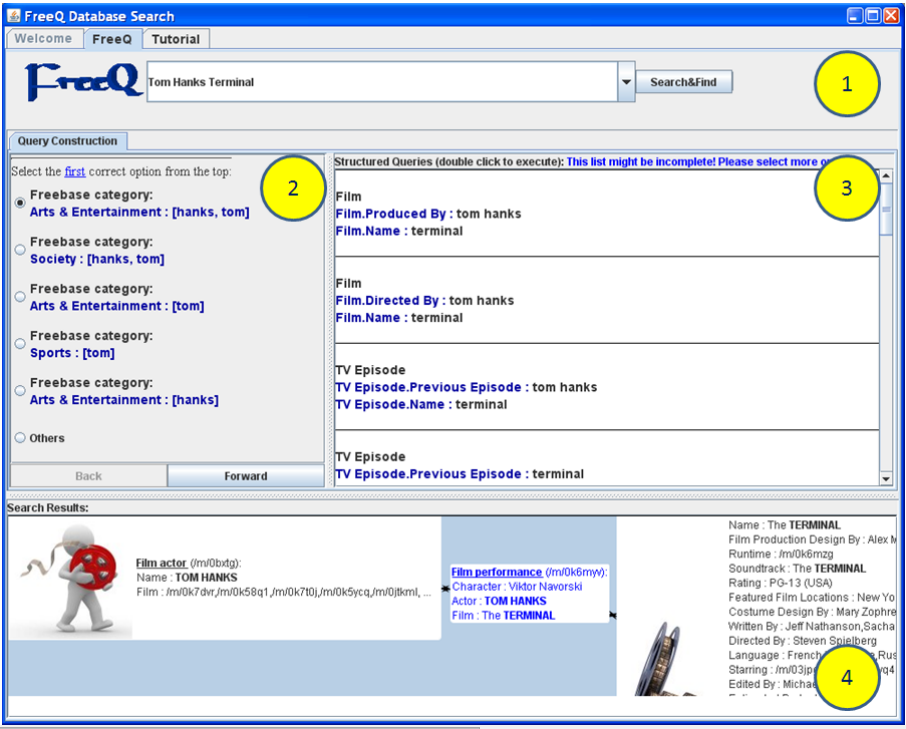
\includegraphics[scale=0.45]{freeq.png}
 \caption{FreeQ GUI. The components of the FreeQ
GUI include: (1) an input field for keyword query,
(2) interaction options, (3) top-k structured queries,
and (4) query results. Attribution: \cite{demidova2012freeq}}
 \label{fig:freeq}
 \end{figure}
 
 When a user issues a keyword query, say \texttt{"Tom Hanks Terminal"}, FreeQ tries to guess the user intent and displays the top-$k$ most likely structured queries in the query window. The user can then click on any of these if it satisfies their information need. 
 
 In the common case, the right structured query will not the identified immediately. The user can then use various interaction options (in the interaction panel) that further clarify intent. These interaction options are simple questions, for example \emph{"Is Tom Hanks a person?"}, and \emph{"Is Terminal an entity in the film domain?"}. Each interaction refines the list of available structured queries to those that comply with the user's selection. 
 
 Conceptually, the main idea is as follows: given a keyword query $K$, the system generates all possible query interpretations of $K$ based on data graph $G$. The set of query interpretations is called the interpretation space of $K$, denoted by $\zeta$. The system also generates a set of interaction options $IO$. If the user selects any interaction option $IO$, the interpretation space $\zeta$ is reduced and further the system displays the top-$k$ interpretations from $\zeta$. The process terminates when the user finds the intended structured query, otherwise it continues generating further interaction options.
 
 It is essential to select the interaction options that can reveal as much information about the user’s intent as possible, i.e., the interaction options with the highest \emph{information gain} need to be identified. FreeQ utilizes the hierarchical conceptual models on top of the database schema to generate interaction options that yield high information gain.
 
 FreeQ extends the Freebase schema with the domain hierarchy of Freebase. Also, FreeQ provides some other types of general interaction options based on hierarchical ontologies. To this end, FreeQ makes use of some external ontologies, such as WordNet \cite{miller1995wordnet} and YAGO \cite{suchanek2007yago}.
 
 The generation of interpretation space is required before top-$k$ interpretations can be obtained. A naive materialization is infeasible for knowledge bases as large as Freebase. FreeQ  uses a query hierarchy introduced in \cite{demidova2012probabilistic}. The hierarchy is grown incrementally during the user interaction phase and generates only the most probable query construction options that comply with the user's selection in each step.
 
 
 
\begin{comment}
\section{Query interpretation based on history}
Fu and Anyanwu [33] propose a context-aware approach for keyword query interpretation that personalizes the interpretation process based on a user’s query context.

In this paper, the problem of generating context-aware query interpretations
for keyword queries on RDF databases by using information from
a user’s query history is addressed. The rationale for this is that users often pose a series of
related queries, particularly in exploratory scenarios. In these scenarios, information
about previous queries can be used to influence the interpretation of a
newer query. For example, given a keyword query “Mississippi River”, if a user
had previously queried about “Mortgage Rates”,then it is more reasonable to
select the interpretation of the current query as being that of a financial institution
“Mississippi River Bank”. On the other hand, if a user’s previous query was
“Fishing Techniques”, it may make more sense to interpret the current query
as referring to a large body of water : the “Mississippi River”. Two main challenges
that arise here include (i) effectively capturing and efficiently representing
query history and (ii) effectively and efficiently exploiting query history during
query interpretation.

The paper proposes and implements a dynamic weighted summary graph model that is
used to concisely capture essential characteristics of a user’s query history.

To achieve this effect, we designed the dynamic weighting function to be
based on a relevance function in terms of two factors: historical impact factor
(hif) and region factor (rf).
Let T indicate the historical index of the most recent query QT , t be the
historical index of an older keyword query Qt, i.e., t $<$ T, and m denote a
summary graph element. Assume that the top-1 interpretation for Qt has already
been generated : QI\textsubscript{t}. Region factor is defined as a monotonically decreasing
function of the graph distance d(m, QIt) between m and QIt:
\begin{align}
rf(d(m, QI\textsubscript{t})) = \frac{1} {a^{d(m,QI\textsubscript{t})}}
\end{align}
Here, a $>$ 1 is a positive integer constant.

Historical impact factor captures the
property that the relevance between a query and a graph element will decrease
when that query ages out of the query history. hif is a monotonically decreasing
function: 
\begin{align}
hif(t) = \frac{1}{b^{T-t}}
\end{align}
where b $>$ 1 is also a positive integer constant.

 
\section{Alternate query languages}
Pound et al. [30] approach the keyword disambiguation problem by ranking different possible rewritings of a query based on their syntactic relationship to the keywords in the query as well as their semantic coherence in the underlying knowledge base. 

In case of unstructured data,
data can be of any type, not necessarily follow any format or rule. e.g. text,video,sound etc. On the other
hand, in case of structured data, the data is organized in semantic chunks(entities). Similar entities are
grouped together to form relations or classes. i.e. in case of structured data, some schema information is
available. As an example ExDB,YAGO have schema items numbering in the millions. So, given such huge
schema information, writing a structured query is a very hard task. This is called Information Overload
Problem. As a naive approach to the above problem, one can use keyword search. But, this comes at a loss of expressivity.
i.e. users can not express desired structure in the query and can not take advantage of schema
information. But, it is very flexible, in the sense that a user can query even if he has no knowledge of the
underlying schema information. On the other hand, conventional structured query is expressive but lacks
flexibility. So, the authors propose a new approach that combines flexibility of keywords as well as expressivity
of structured query, to provide a new query language, called keyword-based structured query
language. e.g. say the information need is “find all people of German nationality who have won a Nobel
award”. Then, the structured query would be
“q(x):- GERMAN PEOPLE(x), hasWonPrize(x, y), NOBEL PRIZE(y)”. The keyword query would be “german
has won nobel award”, and the keyword basedstructured
query would be “german, has won(nobel award)”.


A user enters keyword-based structured query Q to the system. Each keyword k in Q is matched to a set
of schema items using some syntactic similarity measure, with the help of the KB. Each such set forms a
partition. Now, a disambiguation graph G is generated from these. Any induced subgraph of G, that spans
all the partitions, corresponds to a concept query interpretation of Q. Now, these interpretations are ranked
based on some score function that combines semantic and syntactic similarities with the original query Q,
given the KB. Next, top k of those structured queries are evaluated to find potentially relevant entities
and their corresponding documents. The documents are then returned to the user ranked by some relevance
metric.

MashQL [31] present a query formulation language in order to easily query and fuse structured 
data on the web where users can specify filters. It is designed without loss of generality and 
can be used for querying relational databases, XML, RDF and web tables. 

\section{Corpus}
35 propose two new, natural formulations for joint query interpretation and response ranking that exploit bidirectional flow of information between the knowledge base and the corpus.

Here  we  focus  on  a  specific  kind  of  entity  search  query:
Some words (called
selectors
) in the query are meant to occur literally in a response document (as in traditional text
search),  but other words
hint at the type of entity sought
by the query.  Unlike prior work on translating well-formed
sentences or questions to structured queries using deep NLP,
we are interested in handling "telegraphic" queries that are typically sent to search engines.  Each response entity must
be a member of the hinted type.
Note that this problem is quite different from finding answers  to  well-formed  natural  language questions (e.g., in
Wolfram Alpha) from structured knowledge bases (perhaps
curated through information extraction). Also observe that
we do not restrict ourselves to queries that seek entities by
attribute  values  or  attributes  of  a  given  entity  (both  are
valuable query templates for e-commerce and have been re-
searched).   In  our  setup,  some  responses  may  only  be  collected from diverse, open-domain, free-format text sources.
E.g., typical driving
time
between Paris and Nice (the target
type is time duration), or
cricketers
who scored centuries at
Lords (the target type is cricketers).
The  target  type  (or  a  more  general  supertype,  such  as
sportsperson
in place of
cricketer
) may be instantiated in a
catalog
, but the typical user has no knowledge of the catalog
or  its  schema.   Large  catalogs  like  Wikipedia or Freebase
evolve "organically".  They are not designed by linguists, and
they are not minimal or canonical in any sense.  Types have
overlaps  and  redundancies.   The  query  interpreter  should
take advantage of specialized types whenever available, but
otherwise gracefully back o to broader types.


----------------------------
36
We  present  a  new  architecture  for  structural  interpretation of a telegraphic query into these segments:

Mention/s
\^{e\textsubscript{1}}
of an entity
e\textsubscript{1}
,
•
Mention
\^{r}
of a relation type
r
,
•
Mention
\^{t\textsubscript{2}}
of a target type
t\textsubscript{2}
, and
•
Other  contextual  matching  words
s
(some-
times called
selectors
),
with the intent of finding and ranking entities
e\textsubscript{2} $ \in $
t\textsubscript{2}
,  such that
r
(e\textsubscript{1}
, e\textsubscript{2})
is likely
to hold.
Given  the  short,  telegraphic  query  utterances,
we limit our scope to at most one relation mention,
unlike  the  complex  mapping  of  clauses  in  well-
formed  questions  to  twig  and  join  style  queries
(e.g., “find an actor whose spouse was an Italian
bookwriter”). We  present  a  novel  discriminative  graphical
model to capture the entity ranking inference task.

The following notations are used:
\begin{itemize}


\item
$ \Psi $\textsubscript{R}
(q,z,r)
denotes   the   compatibility   be-
tween  the  relation  hint  segment
\^{r} (q,z)
and
a proposed relation type
r
in the KG.
\item 
$ \Psi $\textsubscript{T\textsubscript{2}}
(
q,z,t\textsubscript{2}
)
denotes  the  compatibility  between  the  type  hint  segment
\^{t\textsubscript{2}}
(
q,z
)
and  a
proposed  target  entity  type
t\textsubscript{2}
in  the KG.
\item
$ \Psi $\textsubscript{
E\textsubscript{1}
,R,E\textsubscript{2}
,S}
(
q,z,e\textsubscript{1}
,r,e\textsubscript{2}
)
is a novel corpus-
based evidence potential that measures how
strongly
e\textsubscript{1}
and
e\textsubscript{2}
appear in corpus snippets
in the proximity of words in
\^{s}
(
q,z
)
, and apparently related by relation type
r.
\item
$ \Psi $\textsubscript{
E\textsubscript{1}}
(
q,z,e\textsubscript{1}
)
denotes  the  compatibility  be-
tween the query segment

\^{e\textsubscript{1}}
(
q,z
)
and entity
e\textsubscript{1}
that it purportedly mentions.
\item
$ \Psi $\textsubscript{
S}
(
q,z
)
denotes selector compatibility.  Selectors are a fallback label, so this is pinned
arbitrarily to 1; other potentials are balanced
against this base value.
\item
$ \Psi $
\textsubscript{E\textsubscript{1}
,R,E\textsubscript{2}}
(
e\textsubscript{1}
,r,e\textsubscript{2}
)
is
A
if   the   relation
r
(
e\textsubscript{1}
,e\textsubscript{2}
)
exists in the KG, and is
B $>$
0
otherwise, for tuned/learnt constants
A $>$ B $>$ 0
. Note that this is a soft constraint (
B $>$
0
);
if the KG is incomplete, the corpus may be
able to supplement the required information.
\item
$ \Psi $\textsubscript{
E\textsubscript{2}
,T\textsubscript{2}}
(
e\textsubscript{2}
,t\textsubscript{2}
)
is  1  if
e\textsubscript{2}
belongs  to
t\textsubscript{2}
and
zero otherwise. In other words, candidate
e\textsubscript{2}s
must be proposed to be instances of the proposed
t\textsubscript{2}
— this is a hard constraint, but can
be softened if desired, like
$ \Psi $\textsubscript{E\textsubscript{1},R,E\textsubscript{2}}
\end{itemize}

We perform a MAP inference over all other hidden
variables and note the score of
e\textsubscript{2}
as the product of
the above potentials maximized over choices of all
other variables.\\
score(e\textsubscript{2}) = \\
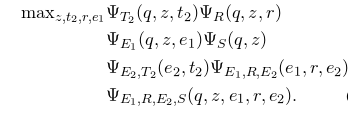
\includegraphics[height=3.5cm]{./1.png}


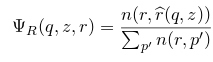
\includegraphics[height=1.5cm]{./2.png}
where
p'
ranges over all phrases that are known to
hint at
r
, and
n
(
r,p
)
denotes the number of sentences where the phrase
p
occurred in the dependency path between the entities participating in relation
r
.

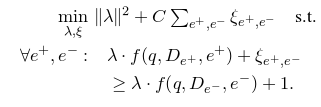
\includegraphics[height=2.8cm]{./3.png}\\
where
e\textsuperscript{+}
and
e\textsuperscript{-}
are positive and negative entities for the query
q
and
f
(
q,D\textsubscript{e}
,e
)
represents the
feature map for the set of snippets
D\textsubscript{e}
belonging
to entity
e
.  The assumption here is that all snip-
pets containing
e\textsuperscript{+}
are “positive” snippets for the
query.
f
consolidates various signals like the number of snippets where
e
occurs near query entity
e\textsubscript{1}
and a relation phrase, or the number of snippets
with high proportion of query IDF, hinting that
e
is a positive entity for the given query.\\

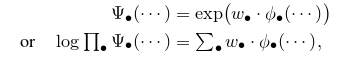
\includegraphics[height=1.8cm]{./4.png}\\

with
w\textsubscript{.}
being a weight vector for a specific potential ., and $ \phi $\textsubscript{.}
being a corresponding feature vector.
During inference, we seek to maximize\\

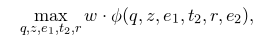
\includegraphics[height=1.5cm]{./5.png}\\

for a fixed
w
, to find the score of each candidate
entity
e
2
.  Here all
w
•
and
φ
•
have been collected
into unified weight and feature vectors
w,φ
. Dur-
ing training of
w
, we are given pairs of correct and
incorrect answer entities
e
+
2
,e
−
2
,  and we wish to
satisfy constraints of the form \\

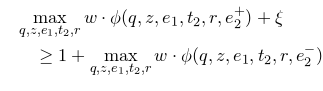
\includegraphics[height=2.3cm]{./6.png}


37
We
propose a structured query mechanism,
entity-relationship
query
, for searching entities in Wikipedia corpus by their
properties and inter-relationships.


\end{comment}